\documentclass{anstrans}
%%%%%%%%%%%%%%%%%%%%%%%%%%%%%%%%%%%
\title{Analysis of the LRA Reactor Benchmark Using Dynamic Mode Decomposition}
\author{Mohammad Abdo, Rabab Elzohery, and Jeremy A. Roberts}

\institute{
Department of Mechanical \& Nuclear Engineering, Kansas State University, Manhattan, KS 66506
}

% Optional disclaimer: remove this command to hide
%\disclaimer{Notice: this manuscript is a work 4of fiction. Any resemblance to
%actual articles, living or dead, is purely coincidental.}

%%%% packages and definitions (optional)
\usepackage{graphicx} % allows inclusion of graphics
\usepackage{booktabs} % nice rules (thick lines) for tables
\usepackage{microtype} % improves typography for PDF
\usepackage{lipsum}
\usepackage{tikz}
\newcommand{\SN}{S$_N$}
\renewcommand{\vec}[1]{\bm{#1}} %vector is bold italic
\newcommand{\vd}{\bm{\cdot}} % slightly bold vector dot
\newcommand{\grad}{\vec{\nabla}} % gradient
\newcommand{\ud}{\mathop{}\!\mathrm{d}} % upright derivative symbol
\DeclareMathOperator*{\argmin}{argmin}

\graphicspath{{../data/images/}}


\begin{document}
%%%%%%%%%%%%%%%%%%%%%%%%%%%%%%%%%%%%%%%%%%%%%%%%%%%%%%%%%%%%%%%%%%%%%%%%%%%%%%%%
\section{Introduction}

The next frontier of reactor modeling will require large-scale, full-core, transient models.
However, the herculean efforts involved will not likely be feasible for applications in which a system model must be executed for multiple system perturbations, e.g., design optimization and uncertainty quantification.
Hence, relatively  inexpensive surrogate models may be needed.

Given access to a high-fidelity model and corresponding solution, data-driven techniques can be used to generate surrogates without resorting to simplified physics or modifying the underlying implementation.  
One class of surrogates recently explored in the nuclear engineering community are those based on dynamic-mode decomposition.  
These past applications involved spatiotemporal dynamics that evolved relatively slowly in time, e.g., the evolution of isotopics \cite{abdo2018data, elzohery2018cbg} and decay-heat generation \cite{alfonsi2018dhc}.

Reactor transients exhibit much different dynamics.
With the restart of TREAT, preliminary efforts to apply surrogates based on generalized polynomial chaos (gPC) for uncertainty quantification have had some success \cite{wang2017usa}.
However, the surrogates generated lacked explicit time dependence and required substantial user development.

Presented here is the development of a data-driven surrogate based on dynamic-mode decomposition (DMD) to approximate time- and space-dependent fluxes and powers.
Specifically, a surrogate was produced for the 2-D LRA transient diffusion benchmark to illustrate the potential of the DMD approach. 
Whereas a conventional DMD surrogate cannot capture the rapid dynamics of the LRA transient, a composite surrogate constructed from a sequence of DMD surrogates defined for successive time windows proved more effective, the details of which are presented below.


\section{Theory}
\label{sec:backgound}

Interest in DMD has grown over the past decade for its ability to represent complex models with explicit temporal dynamics based on observed data alone.  
The basic algorithm was first proposed in the fluid-dynamics community by Schmid for the analysis of experimental data \cite{schmid2010dynamic} but was swiftly developed by others in a variety of fields as has been thorougly detailed in the recent monograph by Kutz {\it et al.} \cite{kutz2016dynamic}.
Underlying the utility of DMD is its strong connection to Koopman theory and the Koopman operator, a linear, infinite-dimensional operator that acts on finite measurements of a nonlinear, dynamical system.
In other words, the Koopman operator provides the machinery to describe the evolution of observations of a nonlinear system in time, and DMD provides a finite-dimensional approximation to this operator.

\subsection{Dynamic Mode Decomposition} 

To motivate DMD, first consider the generic, dynamic problem defined by
\begin{equation}
  \frac{d{\vec{y} }(\vec{r},t)}{dt}=f(\vec{y},\vec{r},t) \, ,
\end{equation}
where ${\vec{y}} \in \mathbb{R}^{n}$ is the $n$-dimensional state vector at time $t$.  
Such a state vector may include neutron fluxes, local powers, temperatures, or functions of such quantities.
Suppose that the evolution of $\vec{y}$ can be well approximated by a relationship of the form  
\begin{equation}
 \frac{d{\vec{y}}(t)}{dt}=\mathcal{A}\vec{y} \, ,
\end{equation}
where the operator $\mathcal{A}$ may not be known explicitly. 
Suppose further that the quantities of interest are sampled at several times and organized as vector of a matrix, i.e.,
\begin{equation}
\mathbf{Y_0}=\left[\begin{array}{ccc}
| & |   & | \\
{\vec{y_0}} &   ... & {\vec{y_{m-1}}} \\ 
| & | &  | 
\end{array} \right] 
 \,\, \text{and} \quad
{\mathbf{Y_1}}=\left[\begin{array}{ccc}
| & |  & | \\ 
{\vec{y_1}} & ... & {\vec{y_{m}}} \\ 
| & |  & |
\end{array} \right] \, ,
\end{equation}
where $m$ is the number of samples (often called snapshots).  
Then
\begin{equation}
  \mathbf{y_{k+1}}=\mathbf{A}\mathbf{y_{k}}, \quad k = 0, 1, \ldots \, ,m-1
\label{eq:snapshot_prop}
\end{equation}
where $\mathbf{A}=\exp(\mathcal{A}\Delta t)$.  
In general, no such operator $\mathbf{A}$ exists such that Eq.~(\ref{eq:snapshot_prop}) is satisfied, and instead, the relation is approximately satisfied by defining
\begin{equation}
\label{eq:AOpt}
    \mathbf{A}=\argmin\limits_{\mathbf{A}}\|\mathbf{Y_{1}} -\mathbf{AY_{0}}\|_F \, ,
\end{equation}
the solution of which is $\mathbf{A}=\mathbf{Y_1}\mathbf{{{Y}_{0}}^{\dagger}}$, where $\dagger$ indicates the pseudoinverse.
However, this matrix is large, and rather than compute it explicitly, the DMD exploits the low-rank approximation
\begin{equation}
\mathbf{\tilde{A}} = \mathbf{U_r^{*}AU_r} \, .
\end{equation}
where $\mathbf{U}_r$ aggregates the first $r$  left singular vectors of $\mathbf{A}$.  Then the eigendomposition
\begin{equation}
 \mathbf{\tilde{A}}\mathbf{W} = \mathbf{W}\bm{\Lambda} \, ,
\end{equation}
approximates the leading $r$ eigenvalues of $\mathbf{A}$ with corresponding 
eigenvectors (often called DMD modes)
\begin{equation}
 \bm{\Phi} = \mathbf{U}_r \mathbf{W} \, .
\end{equation}
Each eigenvalue $\lambda_i$ of $\mathbf{A}$ can be transformed to the continuous frequency $w_i=\log(\lambda_i)/\Delta t$.
Finally, the resulting surrogate is
\begin{equation}
 \mathbf{y}(t) \approx \sum^r_{i=1} \bm{\phi}_i e^{\omega_i t} b_i \, ,
\end{equation}
where the elements of $\mathbf{b}$ are amplitudes of the initial condition in the modal representation.  A typical definition is 
the least-squares representation $\mathbf{b}=\bm{\Phi}^{\dagger} \mathbf{y}_0$.  However, more complicated definitions have been proposed to optimize the representation of the surrogate across all snapshots \cite{jovanovic2014sparsity} and have been employed to support the present effort.

%The procedure is summarized in Algorithm \ref{algDMD}, in which $\vec{b}$ is the amplitude vector computed to satisfy the initial condition in the DMD basis (i.e., $\vec{b}={\boldsymbol{\Phi}^{DMD\dagger}} \vec{y_1}$).

%TODO: add equations for the algorithm.

\subsection{Partitioned DMD}

%TODO: motivate need for time windowing and illustrate basic methodology.

%Maybe ``partitioned DMD''?  
A drawback of DMD is that its modes are non-orthogonal, and hence, increasing the number of modes does not always improve the the prediction because the addition of modes can remove information introduced by previous modes.
Moreover, DMD is known to perform poorly for systems with rapid dynamics.  
Consequently, a simple scheme was explored to improve DMD analysis of rapid dynamics.

Suppose the dynamics of a system can be partitioned into intervals of time in which characteristic time scales are comparable.
Then, DMD can be applied independently within each interval, with ranks selected according to the number of snapshots in the interval and the corresponding dynamics represented by those snapshots.
Identification of partition times can be informed by these underlying dynamics, perhaps as quantified by a mean or integral quantity. 
As an example, it was found for the present work that the core power provided useful guidance.
It is expected that heuristics might exist based on similar, integral in other applications, and that the process of selecting intervals might easily be integrated into an optimization scheme that determines an appropriate threshold value.

\section{Results and Analysis}
\label{sec:application}

\subsection{LRA Benchmark}

The two-dimensional, two-group diffusion LRA benchmark problem is a simplified, quarter-core, BWR model subject to a control-rod ejection with adiabatic heating.
Although complete details can be found elsewhere \cite{anl}, the basic assembly layout is shown in Fig.~\ref{fig:lra_core}.
To produce time-dependent snapshots, the determinstic transport code Detran\footnote{https://github.com/robertsj/libdetran} was used to solve the time-dependent diffusion equations.  
A mesh-centered, finite-volume discretization was used with a 7.5 cm mesh throughout.
A second-order, backward-difference temporal discretization was used with a fixed 0.01 s step size.  
The solution at each time step was converged using fixed-point iteration.
The discretization used is far from numerically converged, but it produces a sufficiently rich set of data for demonstration.

\begin{figure}
\begin{tikzpicture}[scale=.4]

\begin{scope}<->;

% GRID
  \draw[step=1.5cm,gray,very thin, dashed,opacity=0.4] (0, 0) grid (16.5,16.5);

% AXES
  \draw[black, thick, ->] (0, 0) -- (17,  0) node[right] {$x$ (cm)};
  \draw[black, thick, ->] (0, 0) -- ( 0, 17) node[above] {$y$ (cm)};

% Material 1 regions 

  \node[font=\large] at (5.25, 5.25) {1};
  
% Material 2 regions
  \draw[black, thick] (0, 1.5) -- (1.5, 1.5);
  \draw[black, thick] (1.5, 0) -- (1.5, 1.5);
  \node[font=\large] at (0.75, 0.75) {2};
  
  \draw[black, thick] ( 7.5, 0.0) -- ( 7.5, 1.5);
  \draw[black, thick] (10.5, 0.0) -- (10.5, 1.5);
  \draw[black, thick] ( 7.5, 1.5) -- (10.5, 1.5);
  \node[font=\large] at (9.0, 0.75) {2};

  \draw[black, thick] ( 0.0,  7.5) -- ( 1.5,  7.5);
  \draw[black, thick] ( 0.0, 10.5) -- ( 1.5, 10.5);
  \draw[black, thick] ( 1.5,  7.5) -- ( 1.5, 10.5);
  \node[font=\large] at ( 0.75, 9.0) {2};
  
  \draw[black, thick] ( 7.5,  7.5) -- ( 7.5, 10.5);
  \draw[black, thick] ( 7.5,  7.5) -- (10.5,  7.5);
  \draw[black, thick] (10.5, 10.5) -- ( 7.5, 10.5);
  \draw[black, thick] (10.5, 10.5) -- (10.5,  7.5);
  \node[font=\large] at ( 9.0, 9.0) {2};

% Material 3 regions
  \draw[black, thick] (10.5,  0.0) -- (10.5, 10.5) -- (13.5, 10.5) --  (13.5,  0.0) -- (10.5,  0.0);
  \node[font=\large] at ( 12.0, 3.75) {3}; 
  \draw[black, thick] (0.0, 10.5) -- (10.5, 10.5) -- (10.5, 13.5) -- (0.0, 13.5) --  (0.0, 10.5);
  \node[font=\large] at ( 3.75, 12.0) {3}; 
  
% Material 4 regions  
  \draw[black, thick] ( 12,  12) -- ( 12, 10.5) -- (10.5, 10.5) -- (10.5,  12) -- ( 12,  12);
  \node[font=\large] at ( 11.25,11.25) {4};

   
% Material 5 regions
  \draw[black, thick] ( 16.5,  0.0) -- (16.5, 16.5);
  \draw[black, thick] (  0.0, 16.5) -- (16.5, 16.5);
  \node[font=\large] at (15.0, 15.0) {5};
 
% Perturbed regions
  \def\eps{0.125}
  \draw[black, thick, dashed] (10.5+\eps, 7.5+\eps) -- (10.5+\eps, 10.5-\eps) -- (13.5-\eps, 10.5-\eps) -- (13.5-\eps, 7.5+\eps) --  (10.5+\eps, 7.5+\eps);

  %\draw[black, thick] ( 12,  12) -- (10.5,  12);
  %\draw[black, thick] (10.5, 10.5) -- ( 12, 10.5);
  %\draw[black, thick] (10.5, 10.5) -- (10.5,  12);
  \node[font=\large] at (12,9) {R};
 
% ticks
  \foreach \x/\xtext in {15, 75, 105, 120, 135, 165}
      \draw[black,xshift=0.1*\x cm] (0,.3) -- (0,0) node[below] {$\xtext$};
  \foreach \y/\ytext in {15, 75, 105, 120, 135, 165}
      \draw[black,yshift=0.1*\y cm] (.3,0) -- (0,0) node[left] {$\ytext$};
\end{scope}
\end{tikzpicture}
\caption{Schematic of LRA benchmark.  Region numbers indicate material assignment.  Region R is the  ejected rod.  A 15 cm coarse mesh for individual assemblies is overlaid.}
\label{fig:lra_core}
\end{figure}

The initial condition for the transient was computed by solving the steady-state equations, for which the $k_{\text{eff}}$ was found to be 0.9975.
The transient was executed up to 3 seconds.
The space and time discretization employed results in a local (fine-mesh) power distribution of $X \times X$ values recorded at Y times.


\section{Surrogate Generation and Performance}

Snapshots of the mesh-dependent power were extracted from the Detran solution and used as input for the DMD analysis. All DMD analysis presented was performed using modifications of {\tt PyDMD} \cite{demo2018pydmd}.
 
By inspection, it was found that isolation of the transient peak power within a small time interval led naturally to a set of three, partioned DMD surrogates separated at $t = 1.36$ and $t = 1.5$ seconds.  The ranks used in each interval were 10, 13, and 40, each found by an iterative search to minimize the Frobenius norm of the surrogate error in each of the intervals.  Optimized amplitudes (elements of $\mathbf{b}$) were used for the first interval following Ref.~\cite{jovanovic2014sparsity}, while standard projection for the initial condition (i.e., $\mathbf{b}=\bm{\Phi}^{\dagger} \mathbf{y}_0$) was used for the second and third intervals.    The core power density and corresponding absolute, relative error are shown as a function of time in Fig.~\ref{fig:corepower}.  The core power was computed directly from the mesh powers. In addition, mesh powers are shown for $t=0$, $t=1.43$, and $t=2.00$ seconds (i.e., the intial distribution along with the distributions at each peaks) in Fig.~\ref{fig:meshpower}.  


\begin{figure*}[t!]
 \centering
 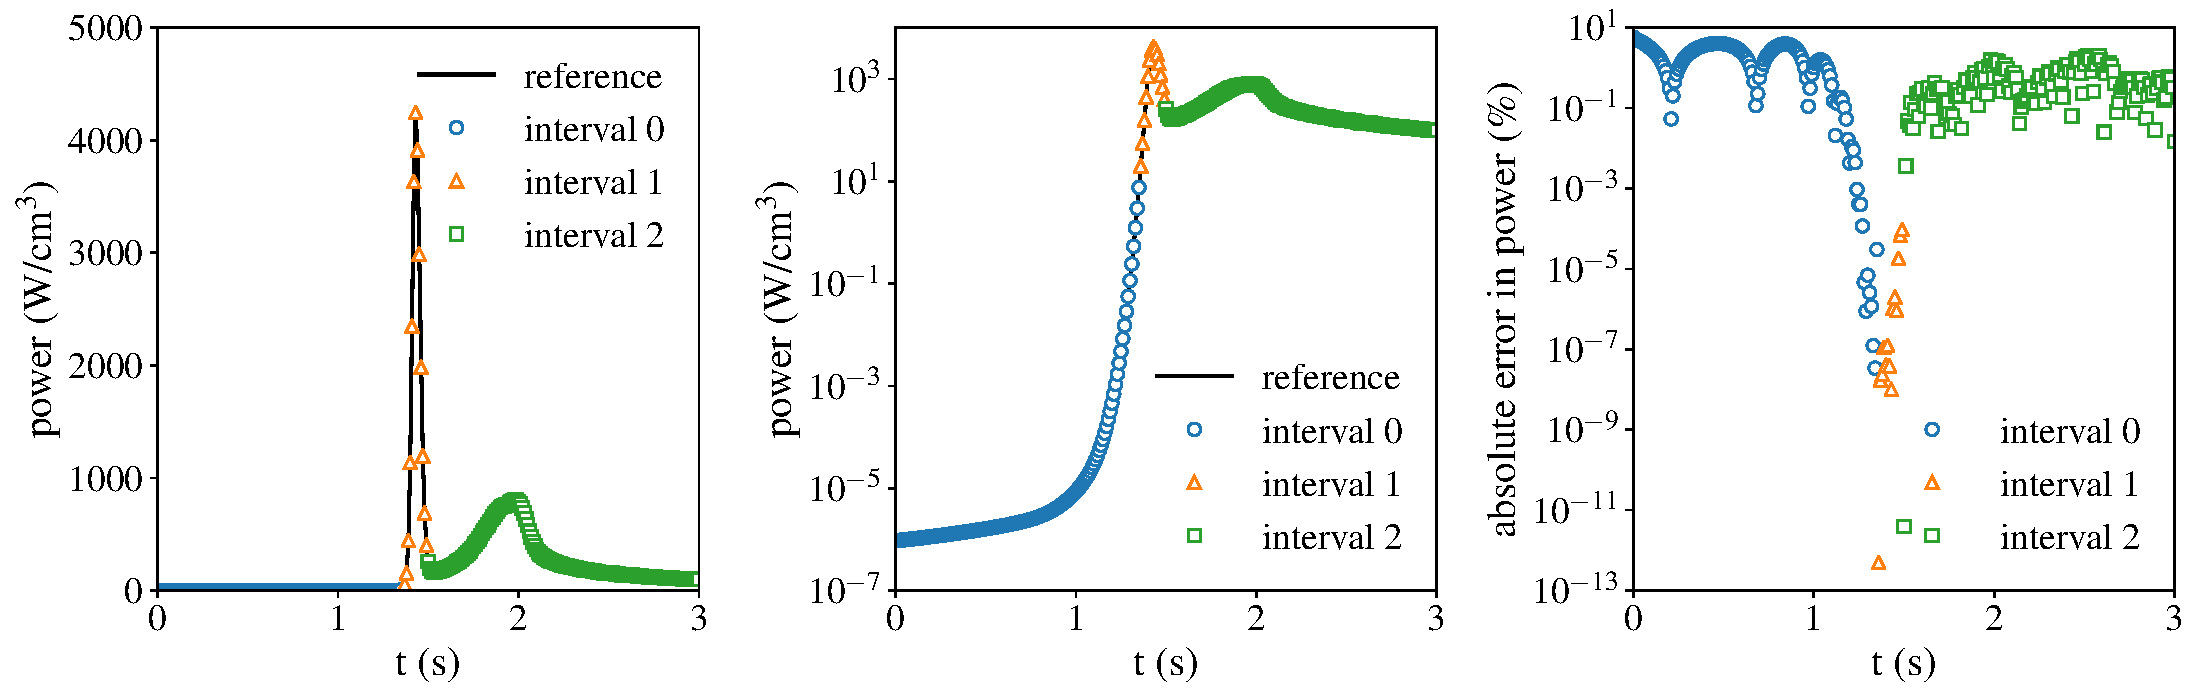
\includegraphics[width=\textwidth]{corepower}\\
   \caption{Left and center: reference and approximate core power density; right: corresponding absolute, relative error.}
  \label{fig:corepower}
\end{figure*}

\begin{figure*}[t!]
 \centering
 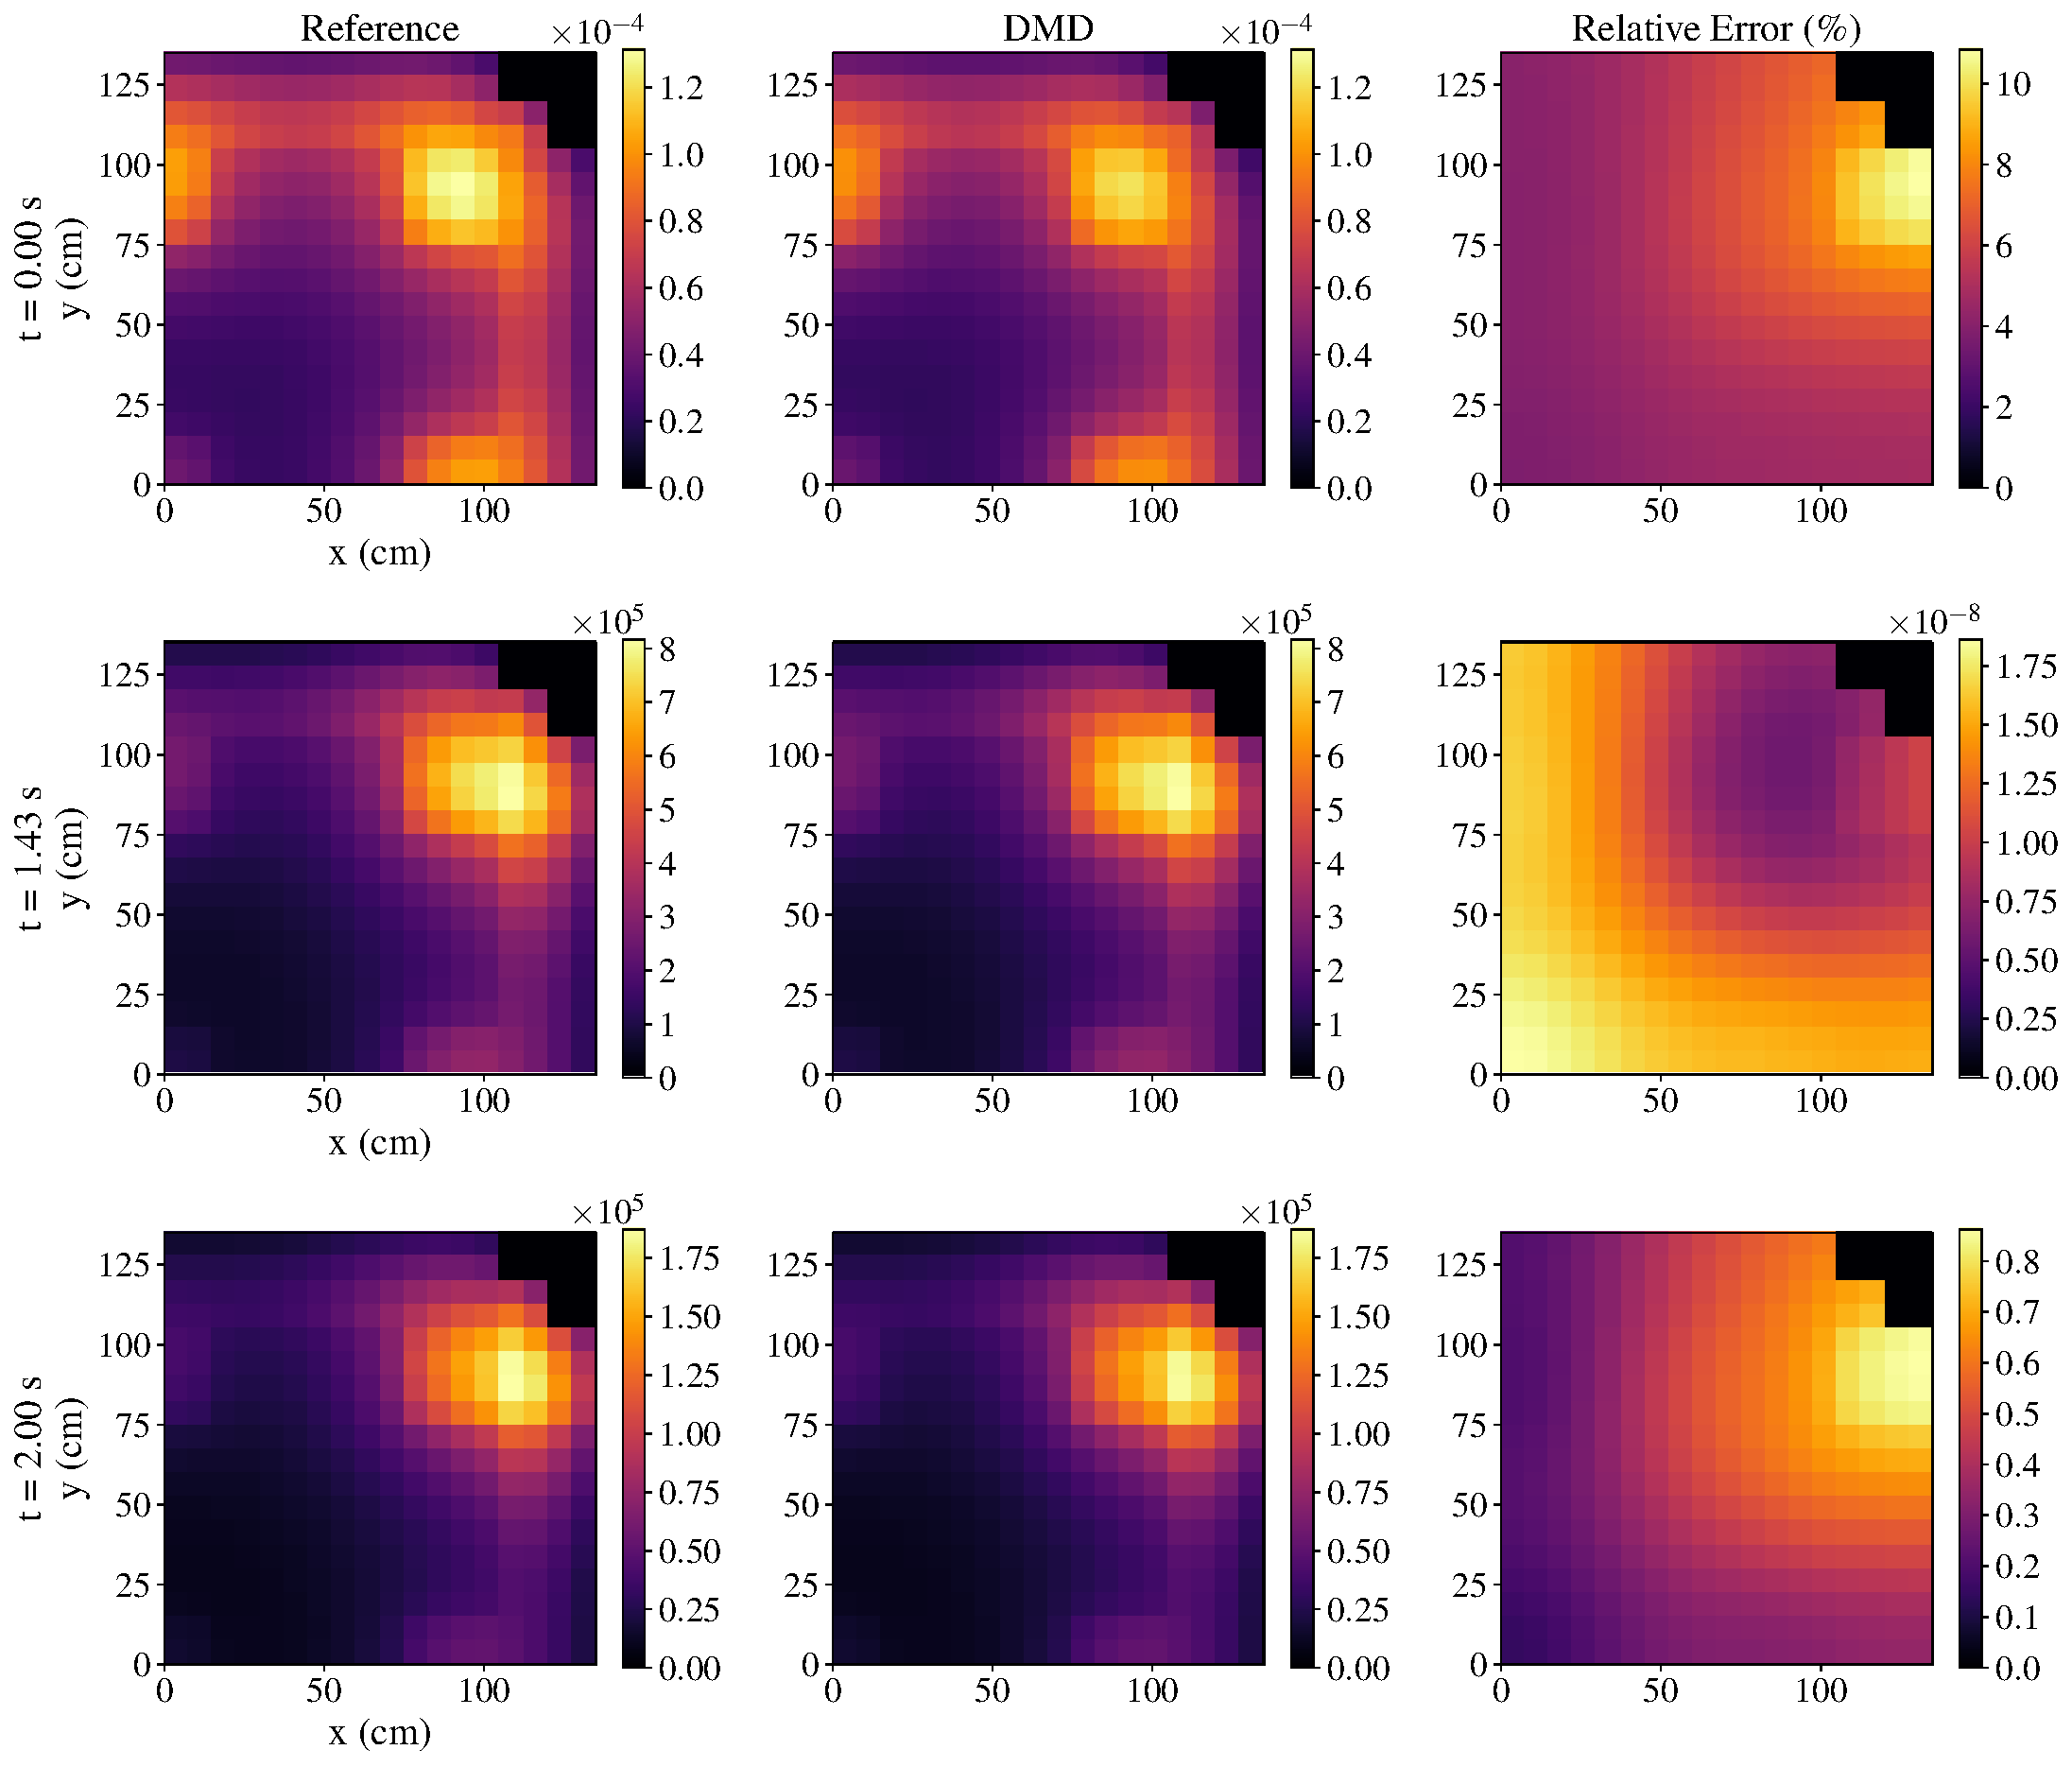
\includegraphics[width=\textwidth]{meshpower}\\
   \caption{Left and center: reference and approximate mesh-wise powers (W); right: corresponding absolute, relative error.}
  \label{fig:meshpower}
\end{figure*}

The surrogate developed reproduces core power with a maximum error of approximately 10\% and much lower errors during the first peak.  The better approximation during the first peak can be attributed at least in part to the smaller time interval.  However, as observed in Fig.~\ref{fig:meshpower}, errors in the mesh powers are very small at the transient peak time of 1.43 s, which suggests the spatiotemporal dynamics through the transient peak are well approximated by a relatively small number of modes.  Errors in power distribution at $t = 0$ and $t = 2$ s are larger.


Though promising, the quality of the approximation proved to be very sensitive to the time intervals, ranks, and amplited vector $\mathbf{b}$ used.  As extreme examples, the removal of just one mode in the second interval increased errors in mesh powers at $t = 1.43$ s from approximately $10^{-7}$ \% to 2.5\%, while the addition of one mode in the third interval led to a solution that grew exponentially in time, a clear indication that the mode added removed important information from the space spanned by the original 40 modes.  These are  significant sensitivities that must be addressed as part of future work, especially if the DMD surrogates are to play a role in quantification of uncertainty.


\section{Conclusions}

A DMD-based surrogate was shown to represent the spatiotemporal dynamics of the LRA benchmark accurately when by produced by a sequence of individual DMD surrogates in time. 
The surrogate was shown to be sensitive to the time partioning.
Work is ongoing to mitigate this sensitivity and to provide an automated way to select the number of partitions and their boundaries.

\section{Acknowledgments}

The material presented is based on work supported in part by a U.S. NRC Faculty Develoment Grant. 

%%%%%%%%%%%%%%%%%%%%%%%%%%%%%%%%%%%%%%%%%%%%%%%%%%%%%%%%%%%%%%%%%%%%%%%%%%%%%%%%
\bibliographystyle{ans}
\bibliography{bibliography}
\end{document}
